%%notwendige packages

%----------------------------

\documentclass[12pt]{article}
%benötigt man immer
\usepackage{amsmath}
%is used for numbering of equations
\usepackage[english]{babel}
\usepackage[utf8x]{inputenc}
\usepackage{varwidth}
\usepackage{float}
% Table caption on top of tables
%\floatstyle{plaintop}
\restylefloat{table}
%----
\usepackage{makecell}
\usepackage{enumitem}

% Für fette Mathesymbole
\usepackage{amsfonts}
\usepackage{amsthm}
\usepackage{bm}
\renewcommand*{\mathbf}[1]{\ifmmode\bm{#1}\else\textbf{#1}\fi}
\usepackage{physics}



% For the type of citation and bibliographic style
%\usepackage{apacite}

% allows index generation
\usepackage{makeidx}
\makeindex

% equation, table and figure numbering should start with section number e.g. (3.1)
\numberwithin{equation}{section}
\numberwithin{table}{section}
\numberwithin{figure}{section}

%fonts
\usepackage[T1]{fontenc}

\usepackage{uarial}
\renewcommand{\familydefault}{\sfdefault}
\usepackage{blindtext}

\usepackage{textcomp}
%\usepackage{mathptmx}
\usepackage{tabularx}
\usepackage{multirow}
\usepackage{enumitem}
%small fonts for captions of figures and tables
\usepackage[center]{caption}
\captionsetup[figure]{font = footnotesize}
\captionsetup[table]{font = footnotesize}


%format
% Witwen und Waisenkinder vermeiden
\clubpenalty=4500	% Waisen vermeiden (erste Zeile eines neuen Absatzes als letzte Zeile einer Seite)
\widowpenalty=10000	% keine Witwen zulassen (letzte Zeile eines Absatzes am Beginn einer neuen Seite)

% Seitenraender einstellen
\usepackage{geometry}
\geometry{a4paper,left=30mm,right=30mm, top=20mm, bottom=20mm}

% Zeilenabstand
\linespread{1.5} 

% Disable indentation for the entire document
\setlength\parindent{0pt}

 % turn off hyphenation and justification
%\raggedright

%Graphics
\usepackage[final]{graphicx} 	
\usepackage[twoside,figuresright]{rotating}
\usepackage{subcaption} 
%\usepackage{subfigure} 

% Adjust tables (and figures) to textwidth...
\usepackage{adjustbox}

%For tables, to color whole row without missing pieces...
\usepackage{tabularx}
%\usepackage[table]{xcolor}  % option loads »colortbl«

% Initialize Makro for table heads
\renewcommand\theadfont{\bfseries\sffamily}

% Highlighting rows, columns and headers of tables
\usepackage{color, colortbl}
\definecolor{Gray}{gray}{0.9}
\definecolor{LightCyan}{rgb}{0.88,1,1}
\definecolor{SeaBlue}{rgb}{0.3, 0.58, 1}

%acronym package for Abbreviations
\usepackage{acronym}

%Create Statutory Declaration page for signatures
\newcommand{\namesigdate}[2][3cm]{%
  \begin{tabular}{@{}p{#1}@{}}
    #2 \\[2\normalbaselineskip] \hrule \\[0pt]
    {\small \textit{Signature}}
  \end{tabular}
}

%----------------------------

\begin{document}

\thispagestyle{empty}	
% !TEX root = Master.tex

%titlepage
\thispagestyle{empty}
\begin{center}


\begin{minipage}{0.75\linewidth}
    \centering
%University logo
    
\includegraphics[scale = 0.7]{figures/uni_goettingen_logo.eps}\\
    
    %\rule{0.4\linewidth}{0.15\linewidth}\par
    \vspace{1cm}
    
% Master Thesis
{{\Huge \textbf{Master Thesis} \par}}
    
\vspace{0.5cm}
    
%Thesis title
    {{\LARGE Multivariate Modelling of the Dependence Structure between Article Sales of a Sportswear Manufacturer\par}}
    \vspace{1cm}
    
    
%Author's name
\begin{center}
Author\\
{\LARGE \textbf{Petros Christanas}} \\
{\large petroschristanas@gmail.com}


\vspace{0.5cm}

Matriculation Number \\
{\large 11604278}

\vspace{1cm}

{\Large Applied Statistics M.Sc.}\\
{\large Chair of Statistics and Econometrics}

\end{center}
    
    \end{minipage}
\end{center}


\vspace{1.5cm}

\noindent Supervisors\\
\noindent {\Large \textbf{Prof. Dr. Thomas Kneib}} \\
\noindent {\Large \textbf{Dipl.-Vw. Quant. Fabian H. C. Raters}} \\

\vspace{0.5cm}
    
%Date
\begin{flushleft}
\noindent {\normalsize Submitted \today} \\
\noindent {\normalsize Processing time of 20 weeks}
\end{flushleft}

    
    

\clearpage


\newpage
\null\thispagestyle{empty}
\newpage
\thispagestyle{empty}
\section*{Confidentiality Clause}
% !TEX root = Master.tex

Write in here the text for the confidentiality clause!

%\clearpage
\newpage
\null\thispagestyle{empty}
\newpage
\thispagestyle{empty}
\section*{Statutory Declaration}
% !TEX root = Master.tex

\vspace{2cm}

I hereby declare that I wrote this thesis paper
independently, without assistance from external parties, and without use of other resources than
those indicated. All information taken from other publications or sources in text or in meaning
are duly acknowledged in the text. The written and electronic forms of the thesis paper are the
same. I give my consent to have this thesis checked by plagiarism software.

\vspace{5cm}

Nuremberg, \today


\vspace{2cm}


\noindent\begin{tabular}{ll}
\makebox[2.5in]{\hrulefill} \\
Petros Christanas \\
\end{tabular}




\newpage
\null\thispagestyle{empty}
\newpage
\thispagestyle{empty}
\section*{Acknowledgments}
% !TEX root = Master.tex

\vspace{3cm}



I would like express my deepest gratitude towards Dr. Alexander März, who guided me throughout this thesis with his expertise and is always finding the time to help during this special times. I would also like to thank the entire adidas Data Science \& AI team for contributing a great deal to my learning journey and giving me the opportunity to conduct this thesis.\\
I am also sincerely grateful towards Prof. Dr. Thomas Kneib for supervising my Master thesis and moreover for leading the study program of Applied Statistics and passing on his knowledge to his students in the best way possible.\\
Last but not least, I would like to thank my fellow students Patrick Neff and Malte Lehna who were playing a key role in my personal growth and with whom I had an unforgettable time in Göttingen. 

\vspace{1.5cm}


\textbf{\textgreekfont{Ευχαριστώ θερμά τους γονείς μου για την άνευ όρων υποστήριξη. Σας αγαπώ!}}



\newpage
\null\thispagestyle{empty}
\newpage


	
%\pagenumbering{Roman} 	
\thispagestyle{empty}
\tableofcontents
\newpage




\newpage

\pagenumbering{arabic} 
\setcounter{page}{1} 

\section{Introduction} \label{introduction}
\input{introduction}
\subsection{Data Sources} \label{data_sources}
% !TEX root = Master.tex

Throughout each season, transactional data are collected from online purchases of the sports brand's e-Commerce website. Specifically, weekly sales data for western European countries consisting of 109 observed weeks in total are provided. A short description is depicted in \autoref{tab:transactional_data}.\\

\begin{table}[H]
\setlength\arrayrulewidth{1pt}  
\centering
\begin{adjustbox}{max width=\textwidth}
\begin{tabular}{|l|l|l|}
\hline
\rowcolor{lightgray} 
\textbf{Column}         & \textbf{Description}                                                                                                        & \textbf{Values}              \\ \hline
week\_id                & Calender week of a specific year (YYYYWW)                                                                         & Factors:\textit{ 201648, ..., 201852}          \\ \hline
article\_number         & Unique article identification number (article ID)                                                                           & Factors: \textit{10669, 10, ...       }        \\ \hline
min\_date\_of\_week     & \begin{tabular}[c]{@{}l@{}} Minimum date of the respective week; always a Monday \\ (YYYY-MM-DD)                                                          \end{tabular} & Dates: \textit{2016-11-28, ..., 2018-12-24}  \\ \hline
art\_min\_price         & Minimal recorded price of the article                                                                                       & Non-negative (integer) value \\ \hline
month\_id               & Calender month of a specific year (YYYYMM)                                                                               & Factors: \textit{201612, ..., 201812}          \\ \hline
season                  & \begin{tabular}[c]{@{}l@{}}Season of year (format: SSYY) \\ (Spring-Summer [SS]:  December - May)\\  Fall-Winter [FW]: June - November)\end{tabular} & \begin{tabular}[c]{@{}l@{}}  Factors: \\ \textit{SS17, FW17,} \\\textit{ SS18, FW18, SS19} \end{tabular} \\

 \hline
bf\_w                   & Weekly "Black Friday" promotion intensity of the article                                                                    & Between \textit{0} and \textit{1}              \\ \hline
ff\_w                   & Weekly "Friends \& Family" promotion intensity of the article                                                               & Between \textit{0} and \textit{1}              \\ \hline
ot\_w                   & Weekly article promotion intensity of "Other" type                                                                          & Between \textit{0} and \textit{1}              \\ \hline
gross\_demand\_quantity & Weekly amount of added articles to shopping cart                                                                            & Non-negative (integer) value \\ \hline
base\_price\_locf       & Retail price of the article without any discounts                                                                           & Non-negative (integer) value \\ \hline
total\_markdown\_pct    &                                                                                                          Total markdown percentage of the article &    Non-negative                           \\ \hline
day\_of\_month          & Day of the month                                                                                                            & Integers: \textit{1 - 31}                       \\ \hline
month\_of\_year         & Month of the year                                                                                                           & Factors: \textit{January, ..., December}       \\ \hline
year                    & Year                                                                                                                        & Integers: \textit{2016, 2017, 2018}             \\ \hline
week\_of\_year          & Week of the year                                                                                                            & Integers: \textit{1 - 52}                       \\ \hline
\end{tabular}
\end{adjustbox}
\caption{Transactional raw data description from online purchases of western European countries}
\label{tab:transactional_data}
\end{table}

Due to legal regulations of the company, some columns had to undergo anonymization in order for the data to be released. To ensure data protection and confidentiality, numeric variables (with exception of time-indicating columns) were transformed. As a consequence for the analysis part, most integer values were converted to float numbers. This fact should be kept in mind by the reader, since the above table serves as a reminder and reference point for the data documentation.\\

Another peculiarity of this setup is to be considered, too. We will often refer to the variable \textit{gross demand quantity} as \textit{sales}, even though it is obviously not exactly the same. In the e-Commerce environment, there are several stages before the purchase is complete, e.g. addition to cart, removal from cart, proceeding to checkout \& even the return of bought articles. Targeting the articles added to cart, i.e. the (gross) demand quantity, provides the optimal data extraction for analytical purposes and is the closest to adequately model the dependence structure between net sales of articles.\footnote{Gross demand quantity will be our target as we follow the adidas norm}  \\

Besides the transactional data, attributes of the articles are provided and described in \autoref{tab:article_master_data}. Some attributes of special importance will be explained in more detail later on in Chapter \ref{sec:data_exploration}. \\

\begin{table}[H]
\setlength\arrayrulewidth{1pt}  
\centering
\begin{adjustbox}{max width=\textwidth}
\begin{tabular}{|l|l|l|}
\hline
\rowcolor{lightgray}
\textbf{Column}           & \textbf{Description}                                   & \textbf{Values (all Factors)}                 \\ \hline
article\_number           & Unique article identification number (article ID)      & \textit{10669, 10, ...}                                \\ \hline
gender                    & Gender type of the article (Men, Women, Unisex)        & \textit{M, W, U}                                       \\ \hline
age\_group                & Age group of the article (Adult, Infant, Junior, Kids) & \textit{A, I, J, K}                                    \\ \hline
key\_category\_descr      & Key category of the article & \textit{KC\_1, ..., KC\_15}   \\ \hline
key\_category\_cluster\_descr      & Key category cluster of the article & \textit{KCC\_1, ..., KCC\_9}   \\ \hline
product\_division\_descr  & Product division of the article                        & \textit{Apparel, Footwear, Hardware}                   \\ \hline
product\_group\_descr     & Product group of the article                           & \textit{Bags, Balls, Footwear Accessories, Shoes, ...} \\ \hline
color                     & Consolidated color group of the article                & \textit{Beige, Black, Brown, Orange, Pink, Red, ... }  \\ \hline
sports\_category\_descr   & Sports category of the article                         & encoded: \textit{SC\_1, ..., SC\_22 }                  \\ \hline
sales\_line\_descr        & Sales line of the article                              & encoded: \textit{SL\_1, ..., SL\_379 }                 \\ \hline
business\_unit\_descr     & The article's Business Unit membership                 & encoded:\textit{ BU\_1, ..., BU\_18   }                \\ \hline
business\_segment\_descr  & The article's Business Segment membership              & encoded: \textit{BS\_1, ..., BS\_49  }                 \\ \hline
sub\_brand\_descr         & Sub-brand of the article                               & encoded: \textit{sub-brand\_1, ..., sub-brand\_4 }     \\ \hline
item\_type                & Item type of the article                               & encoded: \textit{IT\_1, ..., IT\_171 }                 \\ \hline
brand\_element            & Brand element of the article                           & encoded: \textit{BE\_1, ..., BE\_131 }                   \\ \hline
product\_franchise\_descr & Product franchise of the article                       & encoded: \textit{franchise\_1, ..., franchise\_72}     \\ \hline
product\_line\_descr      & Product line of the article                            & encoded: \textit{PL\_1, ..., PL\_105 }                 \\ \hline
franchise\_bin            & Franchise indicator of the article                     &\textit{Franchise, Non-Franchise }                     \\ \hline
category                  & Category of the article                                & encoded: \textit{category\_1, category\_2}             \\ \hline
\end{tabular}
\end{adjustbox}
\caption{Article attribute data}
\label{tab:article_master_data}
\end{table}

%Plenty of additional information is stored in the database, but we are %neglecting columns omitted in these tables, as they are redundant, %already summarized, transformed or simply do not provide any value.\\
Overall, these are the primary data sources and we will be working with data collected over two years, namely the years 2017 and 2018, while some transactions of late 2016 are attached marginally. In summary, after joining the transactional observations to the article attributes by the article ID, this translates to a dataset of 587,127 instances including 26,203 distinct articles and over 30 variables. 


\clearpage

\section{Theory \& Methods} \label{theory_and_methods}
% !TEX root = Master.tex

This chapter introduces some statistical methods used during the conduction of this thesis. Basic notations regarding mathematical foundations of statistics (such as linear algebra, probability theory, hypothesis testing etc) are skipped. Theoretical aspects regarding copulas and dependence structures will be introduced separately in Chapter \ref{sec:copulas_and_dependence_structures}.
%The chapter starts off with some fundamental notions on generalized linear models and arrives at a brief introduction to additive models


\subsection{Generalized Linear Models} \label{glm}
% !TEX root = Master.tex
\textit{\acp{GLM}} are an extension of the classical \textit{\ac{LM}}
\begin{equation}
\begin{aligned}
&y_{i}=\beta_{0}+\beta_{1} x_{i 1}+\ldots+\beta_{k} x_{i k}+\varepsilon_{i}, &i=1, \ldots, n
\end{aligned}
\end{equation}
which in matrix notation can be written as
\begin{equation}
 \bm{y} = \bm{X}\bm{\beta} + \bm{\epsilon} 
\end{equation}
where the response variable $y_i$ can take values from several probability distributions (e.g. Poisson, Binomial, Gamma, ...), which are members of the exponential family \citep{fahrmeir2003regression}. The linear predictor 
\begin{equation} 
\eta_i = \beta_{0}+\beta_{1} x_{i 1}+\ldots+\beta_{k} x_{i k}+\varepsilon_{i} = \bm{x'}_i \bm{\beta} + \bm{\varepsilon}
\label{eq:linear_predictor_glm}
\end{equation}
is passed through a \textit{response function h} (a one-to-one, twice differentiable transformation), such that
\begin{equation}
 E(y_i) = h(\eta_i),
\label{eq:response_function}
\end{equation}
where $h$ ensures that the expected value of the response variable belongs to the appropriate value range. The inverse of the response function, i.e.
\begin{equation}
g = h^{-1},
\label{eq:link_function}
\end{equation} 
is called the \textit{link function} and transforms the mean of the response's distribution to an unbounded continuous scale.

% MAXIMUM LIKELIHOOD ESTIMATION HERE??...




\subsection{Generalized Additive Models} \label{gam}
%input{gam}
\subsection{Mixed Effects Models} \label{mixed_models}
% !TEX root = Master.tex
The \textit{\ac{LMM}} is powerful tool when dealing with clustered data or data with a longitudinal structure (repeated measurements of individuals).
As in the classical \acs{LM}, there are population-specific effects, namely the parameter vector of \textit{fixed effects} $\boldsymbol{\beta}$, as well as the cluster- or individual-specific effects of such models called \textit{random effects} \cite{fahrmeir2003regression}. In the following, we will refer to our clusters or individuals as "groups" for briefness.\ Mathematically speaking, the linear predictor $\eta_{ij}= \mathbf{x}'_{ij} \mathbf{\beta} $ is extended to
\begin{equation}
\eta_{ij} = \bm{{x'}}_{ij} \bm{\beta} + \bm{u'}_{ij}\bm{\gamma}_i, \quad j=1, \ldots, m, \quad i=1, \ldots, n_i, 
\label{eq:linear_mixed_predictor}
\end{equation}
where
\begin{itemize}
\item $i$ is the number of groups
\item $j$ is the number of observations per group
\item $\bm{\beta}$ is the vector of fixed effects
\item $\bm{\gamma}_i$ is the vector of random effects
\item $\bm{x'}_{ij}$ is the vector of covariates and
\item $\bm{u'}_{ij}$ is a subvector of $\bm{x'}_{ij}$.
\end{itemize}


$\bm{x'}_{ij} = (1, x_{ij1}, \ldots, x_{ijk}) $ and $ \bm{u'}_{ij} = (1, u_{ij1}, \ldots, u_{ijk}) $ are therefore the design vectors and $\varepsilon_{ij}$ are the error terms of the \textit{measurement model}

\begin{equation}
y_{ij} =  \bm{x'}_{ij} \bm{\beta} + \bm{u'}_{ij} \bm{\gamma}_i + \epsilon_{ij}, \quad \varepsilon_{i j} \overset{i.i.d.} \sim N\left(0, \sigma^{2}\right) 
\end{equation}
or in matrix notation

\begin{equation}
\bm{y}_{i}=\bm{X}_{i} \bm{\beta} + \bm{U}_{i} \bm{\gamma}_{i} + \bm{\varepsilon}_{i}
\end{equation}
for group $ i=1, \ldots, m $ with $ E(\bm{\varepsilon}_{i}) = \bm{0}$. \\

Similar to \ac{GLM}s, the \textit{\ac{GLMM}} relates the linear mixed predictor \ref{eq:linear_mixed_predictor} to the conditional mean 
$ \mu_{ij} = E(y_{ij} | \bm{\gamma}_{i}) $
via a suitable response function $h$, such that
$ \mu_{ij} = h(\eta_{ij}) $ and thus the conditional density of $y_{ij}$ belongs to the exponential family.
%\input{random_intercept_model}



\clearpage

\section{Study Area \& Data Sources}
\subsection{Forest Classification}
% !TEX root = Master.tex

The study area is a private forest enterprise in Gartow (Niedersachsen) Germany. It measures around 5674.2 ha in total (see Table \ref{tab:sizes}) and is a relatively homogenous forest consisting mostly of pine trees.

\begin{table}[H]
\setlength\arrayrulewidth{1pt}  
\centering
\begin{tabular}{|c |c |c |c|}
\hline 
\rowcolor{Gray}
\textbf{Stratum} & \textbf{Location Class} & \textbf{Area [ha]} & \textbf{Relative Area} \\ 
\hline 
1 & 1 & 338.6 & 0.06 \\ 
\hline 
2 & 2 & 1546.9 & 0.27 \\ 
\hline 
3 & 3 & 2129.3 & 0.38 \\ 
\hline 
4 & 4 & 1550.5 & 0.27 \\ 
\hline 
G & 2 & 108.9 & 0.02 \\ 
\hline 
\rowcolor{SeaBlue}
Total & - & 5674.2 & 1 \\ 
\hline 
\end{tabular} 
\caption{Size of the different stratum and associated sampling grids. Stratum 2 and G have been merged to Location Class 2 which results in an identical sampling grid.}
\label{tab:sizes}
\end{table}

The forest itself is split into stratum to take site conditions, forest structure and thus natural variation of the areas into account (see Figure \ref{fig:Gartow Map}). The assessment of variation was based on a forest inventory conducted 2008
(see Table \ref{tab:Sample_Variation}).

\begin{table}[H]
\setlength\arrayrulewidth{1pt}  
\centering
\begin{adjustbox}{max width=\textwidth}
\begin{tabular}{|c |c |c |c |c |c |c |c|}
\hline 
\rowcolor{Gray}
\textbf{Stratum} & \textbf{Location Class} & \textbf{Area [ha]} & \textbf{Relative Area} & \textbf{Sample Size} & \textbf{Mean Volume / ha} & \textbf{Sample Variance} & \textbf{SE\%} \\ 
\hline 
1 & 1 & 338.6 & 0.06 & 159 & 180.19 & 104.24 & 5.67 \\ 
\hline 
2 & 2 & 1546.9 & 0.27 & 805 & 246.75 & 22.75 & 1.93 \\ 
\hline 
3 & 3 & 2129.3 & 0.38 & 542 & 195.41 & 13.15 & 1.86 \\ 
\hline 
4 & 4 & 1550.5 & 0.27 & 134 & 131.90 & 30.45 & 4.18 \\ 
\hline 
G & 2 & 108.9 & 0.02 & 55 & 271.26 & 734.08 & 9.99 \\ 
\hline 
\rowcolor{SeaBlue}
Total & - & 5674.2 & 1 & 1659 & 196.37 & 6.46 & 1.29 \\ 
\hline 
\end{tabular} 
\end{adjustbox}
\caption{Mean volume and sample variation estimates of the forest inventory 2008. Stratum 2 and 3 show little relative standard
error (SE\%), while stratum 1 inhibits more variation. Stratum G, which covers only 2\% of the total area has a typical high variation}
\label{tab:Sample_Variation}
\end{table}

Main sources of the variation in the growing stock can be assigned by the varieties in the tree species and the age distribution of the trees. Young and therefore small trees have a smaller diameter. If an area has been cultivated around the same timespan with identical species, the trees are expected to be centred on a certain diameter. On the other hand, a very diverse area in species and time will have naturally more variation (see Figure \ref{fig:barplots_Gartow})

\begin{figure}[H]
  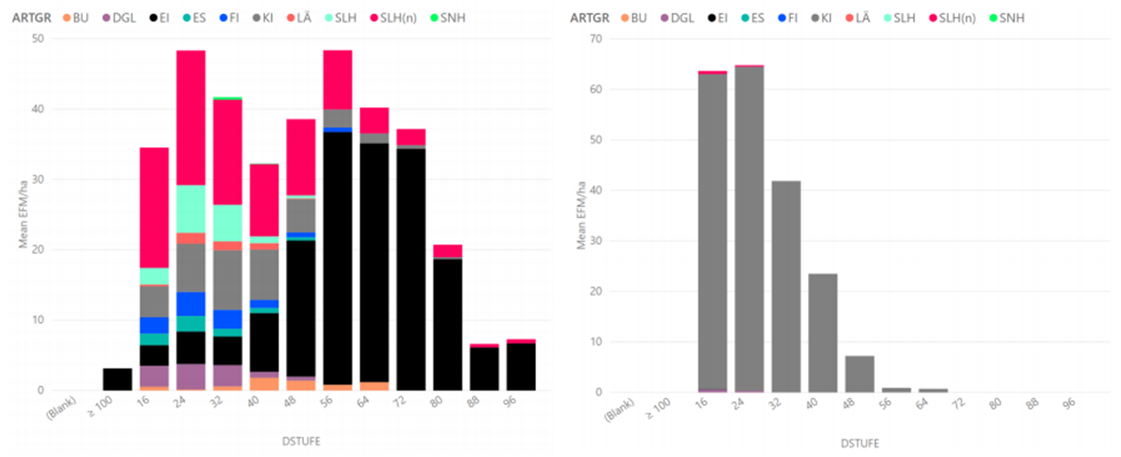
\includegraphics[width=\textwidth]{barplots_Gartow.png}
  \caption{The bar plots (left to right: stratum 1, stratum 4). The bars indicate the mean volume per ha for different diameter classes [1].}
  \label{fig:barplots_Gartow}
\end{figure}

Sampling activities are adjusting according to the inhibited variation of the stratum type (see Section \ref{Inventory Data}).

\begin{figure}[H]
  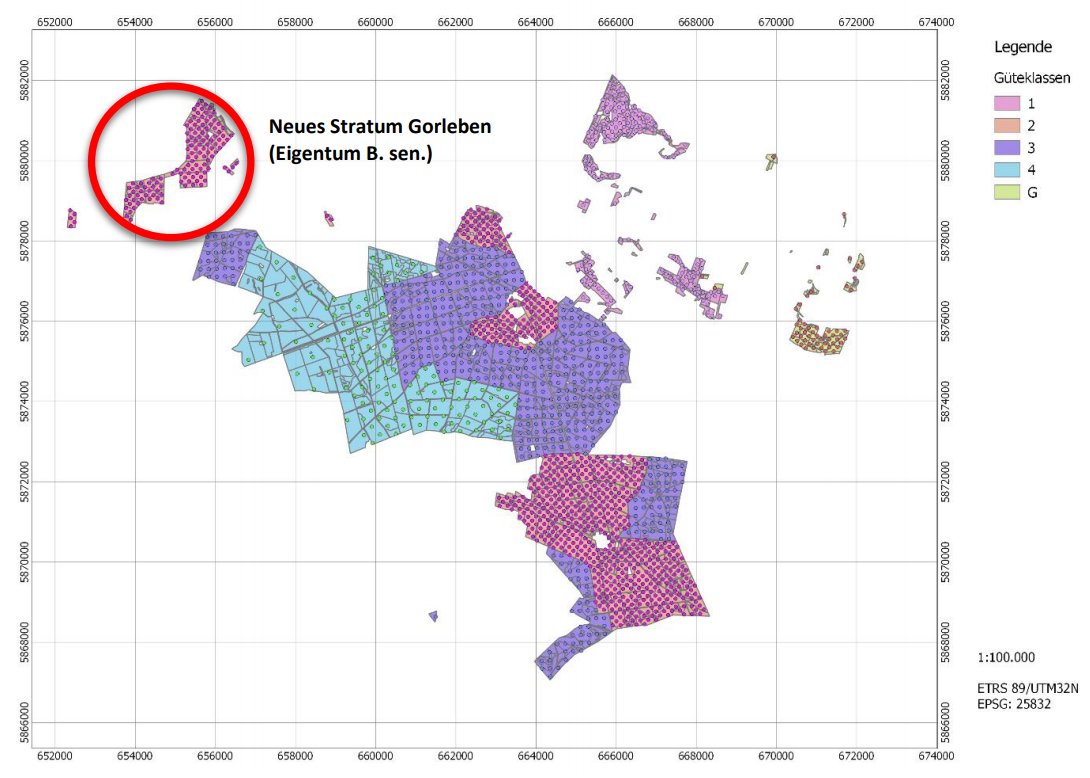
\includegraphics[width=\textwidth]{Gartow_map.png}
  \caption{The forest of Gartow is divided into stratums based on past observed variation and ownership and subdivided into compartments indicated by grey lines. Each point within a section indicate a sampling point [1].}
  \label{fig:Gartow Map}
\end{figure}

The stratum themselves are subdivided into compartments with the intention to create homogeneous sub regions (see Figure \ref{fig:Gartow Map}). The diameter distribution must be found for each of those compartments.

\subsection{Inventory Data} \label{Inventory Data}
% !TEX root = Master.tex

In spring 2018, a sample-based forest inventory was carried out in Gartow. 942 sampling locations are defined which are spread over the forest based on a stratified sampling approach. This accounts for the past observed variation within the regions. Compartments of stratum 1 and 2 are sampled with a dense sampling grid, while 3 and 4 have a wider sampling grid (see Table \ref{tab:Sample_Variation} \& Figure \ref{fig:Gartow Map}).\\

At each sampling location (so called plots) several attributes of the trees within a certain circular area are measured. The parameters of primary interest in this study are the diameter, species and height. The diameter is measured at breast height (around 1.3 meters) with a measuring tape. Subsequently, the height is measured with varying, but established methodologies. Unlike the diameter, not every tree height is collected. In each plot, three main species trees (less if there are fewer trees) are measured. To cover the total range of values, a small, a medium sized and a large one is gauged. Additionally, one tree of every other species is measured to cover the variety of species. Table \ref{tab:Measured Trees} provides an overview of total measured trees.

\begin{table}[H]
\setlength\arrayrulewidth{1pt}  
\centering
\begin{tabular}{|c| c|}
\hline 
\rowcolor{Gray}
\textbf{Stratum} & \textbf{\# Measured Trees} \\ 
\hline 
1 & 1287 \\ 
\hline 
2 & 3434 \\ 
\hline 
3 & 2734 \\ 
\hline 
4.1 & 616 \\ 
\hline 
4.2 & 792 \\ 	
\hline 
G & 523 \\ 
\hline 
GL & 619 \\ 
\hline 
\rowcolor{SeaBlue}
Total & 10005 \\ 
\hline 
\end{tabular} 
\caption{Overview of number of measured trees for height and diameter per Stratum}
\label{tab:Measured Trees}
\end{table}


\subsection{LiDAR} \label{LiDAR}
% !TEX root = Master.tex

While the previously described data will be used for modelling, data captured by the airborne LiDAR is of main interested in this report, since the ability of innovating forest inventory is discussed.\\

LiDAR uses a laser scanning system to capture distances. In context, laser scanning is referred to the active emitting and sensing of light. Thus, Light Detection and Ranging is a suitable description of the mechanics, also known as LADAR (Laser Detection and Ranging). LiDAR is a more generalized definition, as instead of laser- light also xenon or flash lamps can be used [2]. A high-level definition of the functionality of LiDAR is as follows. Laser beams are continuously emitted of the LiDAR system, mounted on an airborne vehicle. The coordinates are throughout captured by a GPS (Global Positioning System) and IMU (Inertial Measurement Unit – used to capture adjust for e.g. inclined positioning, acceleration of the vehicle). Laser or xeon/flash light is emitted of an active sensor and the distance captured once it is traveled back to the scanner. As forests have a relatively turbulent surface and only little light can reach the surface of the forest, many systems only capture the first and last impulse [3]. The cloud of captured points can then be used to create a 3-D image of the forest (see Figure \ref{fig:LiDAR}).

\begin{figure}[H]
  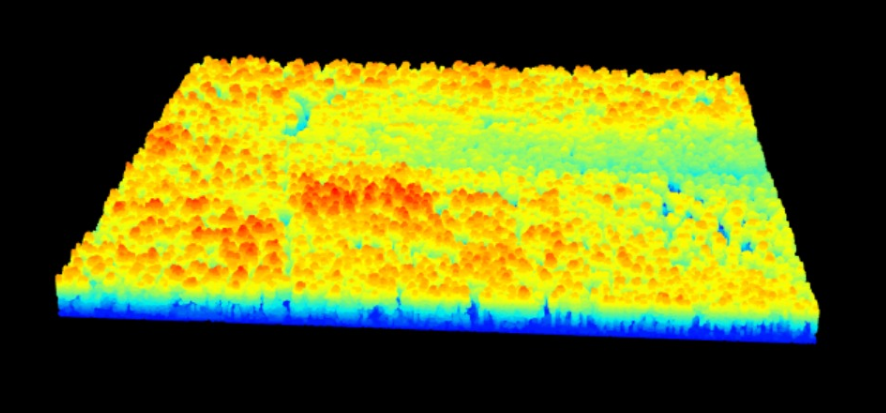
\includegraphics[width=\textwidth]{lidar.png}
  \caption{3-D Image of a small area of the forest of Gartow made by the airborne LiDAR. The determined height is colorized. A
dense group of height trees is found almost in the middle and directly behind an aisle of small trees.}
  \label{fig:LiDAR}
\end{figure}

Main benefits of LiDAR compared to other systems is the ability to capture data regardless of sun positioning, day or night and the ability to map through the highly dense areas (the canopies of the trees). The main benefit compared to the traditional way of forest inventory is relative intuitive. A plane is capable of objectively measuring the forest subject to this report in under a week; while a forester must inspect every single hectare, providing a more subjective intuition of the forest inventory.

\begin{table}[H]
\setlength\arrayrulewidth{1pt}  
\centering
\begin{adjustbox}{max width=\textwidth}
\begin{tabular}{|c|c|}
\hline
\rowcolor{Gray}
\textbf{Flight Altitude}              & \textbf{Approx. 590m above ground} \\ \hline
Nominal point density (laser)         & 6 points / m²                      \\ \hline
Ground resolution                     & 4.3cm                              \\ \hline
Point density (to circumvent overlap) & 12 points / m²                     \\ \hline
Ground resolution                     & 4.3cm                              \\ \hline
\end{tabular}
\end{adjustbox}
\caption{Flight log of the airborne laser scanning of the forest of Gartow [12]}
\label{tab:Flight log}
\end{table}

ForestEye Research GmbH \& Co. KG provided the detected single tree location, tree species and canopy area based on LiDAR.
\clearpage


\section{Data Exploration} \label{Data Exploration}
% !TEX root = Master.tex

Let's begin with the data exploration


$$\hat{\beta}^{\text {ridge}}=\underset{\beta}{\arg \min }\left((y-X \beta)^{\prime}(y-X \beta)+\lambda \sum_{j} \beta_{j}^{2}\right)$$
jkhnvcv
\clearpage

\section{Conclusion} 
\input{Conclusion}
\clearpage



\addcontentsline{toc}{section}{Appendix}
\section*{Appendix} \label{Appendix}
% !TEX root = Master.tex

Include appendix here...

\clearpage



\addcontentsline{toc}{section}{List of Figures}	
\listoffigures


\clearpage

\addcontentsline{toc}{section}{List of Tables}
\listoftables


\clearpage

\addcontentsline{toc}{section}{List of Abbreviations}
\section*{List of Abbreviations}
% !TEX root = Master.tex

\begin{acronym}
 
\acro{aka}{Also known as}
\acro{BIC}{Bayesian Information Criterion} 
\acro{GLM}{Generalized Linear Model}
\acro{LM}{Linear Regression Model}
\acro{LMM}{Linear Mixed Model}
\acro{GLMM}{Generalized Linear Mixed Model}
\acro{CDF}{Cumulative Distribution Function}
\acro{PDF}{Probability Density Function}
\acro{RV}{Random Variable}
\acro{wlog}[w.l.o.g.]{Without loss of generality}
\acro{dof}[d.o.f.]{Degrees of Freedom}
\acro{GAM}{Generalized Additive Model}

\end{acronym}





\clearpage

\addcontentsline{toc}{section}{References}
% MAKE THE REFERENCES PROPER; CITATIONS ETC....
% Insert bibliography and the bibliographic style
\bibliographystyle{apalike}
\nocite{*}
\bibliography{references}

\end{document}

